 \documentclass[a4paper,12pt]{article}
\usepackage[a4paper,top=3cm,bottom=2cm,left=3cm,right=3cm,marginparwidth=1.75cm]{geometry}
\usepackage[brazil]{babel}
\usepackage[T1]{fontenc}
\usepackage[utf8]{inputenc}
\usepackage{amsmath}
\usepackage{MnSymbol}
\usepackage{wasysym}
\usepackage{hyperref}
\usepackage{color}
\definecolor{Blue}{rgb}{0,0,0.9}
\definecolor{Red}{rgb}{0.9,0,0}
\usepackage{esvect}
\usepackage{graphicx}
\usepackage{float}
\usepackage{indentfirst}
\usepackage{caption}
\usepackage{blkarray}
\newcommand\Mark[1]{\textsuperscript#1}
\usepackage{pgfplots}
\usepackage{amsfonts}
\usepackage[english, ruled, linesnumbered]{algorithm2e}
\usepackage{algorithmic}
\newtheorem{definicao}{Definição}[section]
\newtheorem{teorema}{Teorema}[section]

\title{Teoria de Grafos}
\author{Guilherme Philippi, Felipe Delfini Caetano Fidalgo}
\begin{document}
\maketitle
\tableofcontents

\section{Teoria de Grafos\label{sec:grafos}}
Esta seção tem como objetivo apresentar um breve resumo da \textit{teoria de grafos}, tema muito estudado por diversos matemáticos e aplicado em diversas áreas do conhecimento \cite{GraphTheoryApplicationsBondy}.

\subsection{Descoberta (Eureka!)}
Costuma-se dizer que em 1736 é que a teoria teve início, com base no artigo publicado por Leonhard Euler sobre as 7 pontes de Königsberg \cite{euler:KOENIGSBERG} \cite{GraphTheoryApplicationsBondy}, representada na Figura~\ref{fig:koni}. Esse é um problema muito usado para introduzir o tema didaticamente --- propõe-se o desafio de ligar todos os pontos de um desenho sem tirar o lápis do papel e sem passar duas vezes no mesmo ponto. Segundo a história, os moradores daquela região perguntavam-se sobre a possibilidade de atravessar todas as sete pontes do local sem ter que repetir alguma delas. Euler provou que isso não era possível ao formular matematicamente o problema, que deu origem a esta teoria.

\begin{figure}[H]
	\begin{center}
		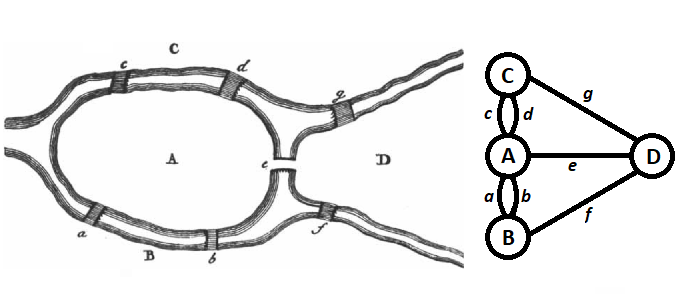
\includegraphics[width=0.7\linewidth]{koenigsbern.png}
	\end{center}
	\caption{Ilustração original do problema \cite{euler:KOENIGSBERG}.}
	\label{fig:koni}
\end{figure}

A grande ideia de Euler foi abstrair o problema, vê-lo de uma forma elementar, como um conjunto de pontos conectados por curvas (representado por um "gráfico", conforme Figura~\ref{fig:koniGrafo}). Essa representação facilita a análise e a busca por uma solução. Logo Euler percebeu que só seria possível solucionar o problema se houvessem exatamente nenhum ou apenas dois pontos conectados por um número impar de curvas (ou pontes) \cite{euler:KOENIGSBERG}. Note que o caso de Koenigsberg não respeita essa característica.

\begin{figure}[H]
	\begin{center}
		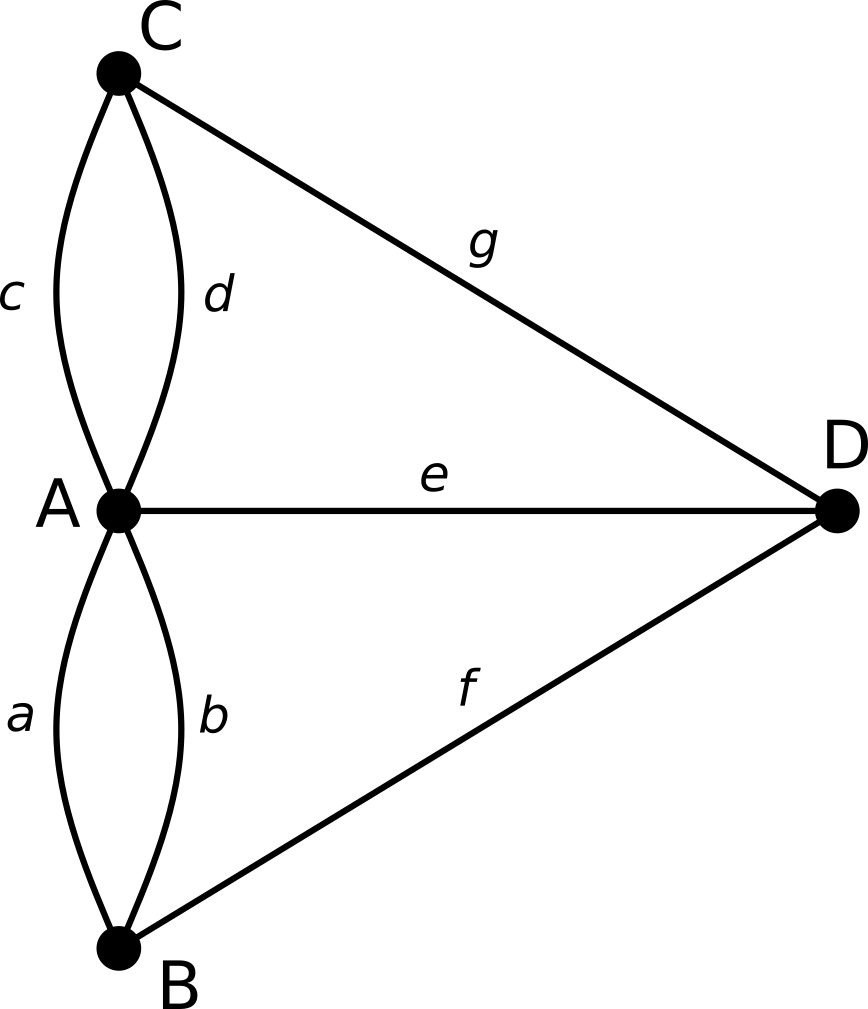
\includegraphics[width=0.35\linewidth]{koenigsbernGrafo.png}
	\end{center}
	\caption{Representação em Grafos da ponte de Koenigsberg.}
	\label{fig:koniGrafo}
\end{figure}

Mas não podemos deixar todo o mérito com Euler. O conceito de grafo é muito intuitivo e foi proposto por diversas mentes brilhantes como formas de solucionar problemas que, em sua essência, são muito parecidos. Após Euler, a teoria foi redescoberta por Kirchhoff e Cayley \cite{graphTheoryFHarary}. Kirchhoff desenvolveu a teoria por volta de 1847, enquanto solucionava sistemas de equações lineares que relacionavam as correntes que passavam em cada malha fechada de um circuito elétrico \cite{kirchhoff1847ueber}, seguido por Cayley, em 1857, que estudava diferentes estruturas em bioquímica formadas por carbonos (sempre com quatro ligações químicas) e hidrogênios (com apenas uma ligação), onde conseguiu formular seu problema introduzindo o conceito de \textit{árvore} em grafos \cite{cayley1897theory}.  

Além dessas, muitas outras situações reais podem ser convenientemente representadas por simples diagramas contendo um conjunto de pontos e um conjunto de relações entre pares desses pontos. Por exemplo, podemos definir o conjunto $P = \{a,b,c\}$ das pessoas $a, b$ e $c$ e um conjunto $A = \{\{a,b\}, \{b,c\}\}$ como o conjunto de amizades entre essas pessoas --- no caso, $a$ é amigo de $b$, que é amigo de $c$, porém $a$ não é amigo de $c$. 
Este exemplo se torna muitíssimo útil quando se deseja estudar como a informação se propaga em redes sociais.

\subsection{Definição}

Não há um forte consenso sobre as terminologias usadas pelos autores quando se define sobre grafos \cite{graphTheoryFHarary}. Essa confusão é tanto gerada pela vasta disseminação da teoria em diversas áreas como pela enorme abstração que ela carrega. Cayley poderia chamar as relações entre pontos de ligações químicas enquanto Kirchhoff chamaria de curto-circuitos.

Fazer-se-há aqui um apanhado de definições sobre a teoria de grafos, mas não sobre toda ela. Essa é uma grande área da matemática e não nos cabe aborda-lá completamente aqui. Trata-se apenas do essencial para que o leitor possa progredir sem ter que consultar uma bibliografia complementar sobre grafos.

\begin{center}
	\begin{minipage}{0.9 \linewidth}
		\textbf{Grafo:} Um grafo $G$ é uma tripla ordenada da forma $(V(G),E(G), \psi_{G})$, composto por um conjunto de \textit{vértices} $V(G)$, de arestas $E(G)$ e uma \textit{função de incidência} $\psi_{G}$ que, por sua vez, associa a cada aresta de $V(G)$ um par não ordenado de vértices (nem sempre distintos) de $E(G)$. Costumamos dizer que as arestas ligam os vértices.
	\end{minipage}
\end{center}

Existe, também, uma íntima relação entre Grafos e algoritmos. De fato, podemos inclusive representar um algoritmo por um grafo \cite{grafos0}. Na verdade, a definição de grafos é tão abrangente que podemos ver suas ligações com diversas áreas do conhecimento. 

Daí vem o seu nome em inglês: "Graph", que, em tradução livre, é "gráfico"

No que se segue, definiremos algumas características elementares que serão utilizadas durante esse texto. Para um estudo mais completo sobre essa teoria, vide \cite{grafos1} e \cite{grafosPremioElon}.

\subsection{Algumas Classificações Importantes}

Existem duas definições de extrema importância para o nosso problema molecular (tema central desse texto): o conceito de grafo completo e o de estruturas $k$-cliques. Porém, seremos obrigado a definir alguns outros conceitos prévios, como segue. 


\begin{center}
	\begin{minipage}{0.9 \linewidth}
		\textbf{Laço:} Uma aresta $\{e_i, e_j\} \in E$ tal que $i = j$.
	\end{minipage}
\end{center}

Também, caso existam duas arestas iguais ($\{e_i, e_j\}$ e 
$\{e_j, e_i\}$, por exemplo, lembrando que $E$ é um conjunto de pares não ordenados), com as mesmas extremidades, estas recebem o nome de \textbf{arestas paralelas}.

\begin{center}
	\begin{minipage}{0.9 \linewidth}
		\textbf{Grafo simples}: Um grafo que não possui laços ou arestas paralelas.
	\end{minipage}
\end{center}

\begin{center}
	\begin{minipage}{0.9 \linewidth}
		\textbf{Grafo Completo:} É um grafo simples em que todo vértice é conectado a todos os outros vértices.
	\end{minipage}
\end{center}

\begin{figure}[H]
	\begin{center}
		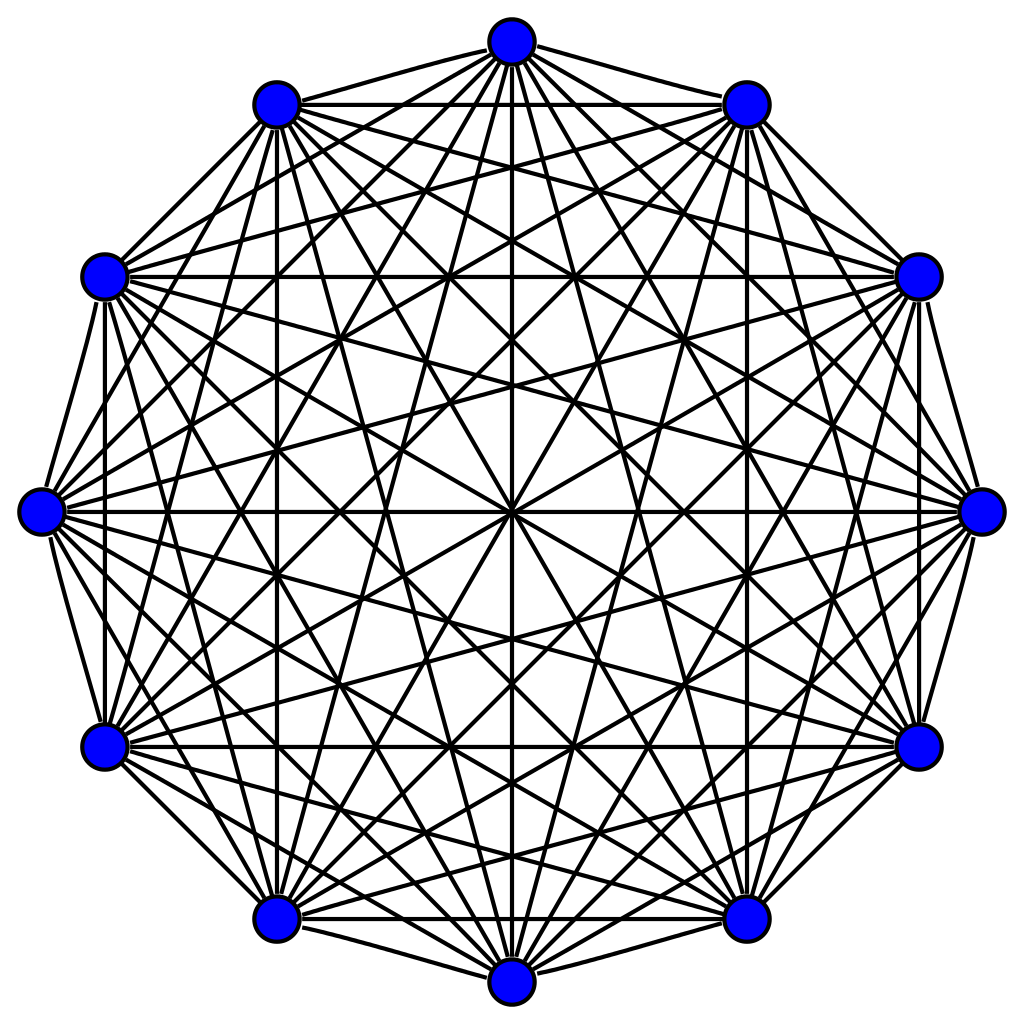
\includegraphics[width=0.4\linewidth]{grafocompleto.png}
	\end{center}
	\caption{Diagrama de um grafo completo com 12 vértices ($|V| = 12$).}
	\label{fig:grafocompleto}
\end{figure}

Outro conceito que nos será de grande utilidade é o de subgrafo.
\begin{center}
	\begin{minipage}{0.9 \linewidth}
		\textbf{Subgrafo:} É um grafo resultante de um subconjunto de vértices e outro subconjunto de arestas de outro grafo. Isto é, seja $G = (V, E), G^\prime = (V^\prime, E^\prime)$ é dito um subgrafo de $G$ se $(V^\prime, E^\prime)$ é um grafo tal que $V^\prime \subseteq V$ e $E^\prime \subseteq E$.
	\end{minipage}
\end{center}

E, finalmente
\begin{center}
	\begin{minipage}{0.9 \linewidth}
		\textbf{$k$-Clique}: é um subgrafo $G^\prime$ com $k$ vértices tal que $G^\prime$ é completo.
	\end{minipage}
\end{center}

Em especial, também podemos interpretar as arestas como \textit{caminhos} e, se o fizermos, podemos pensar em alguma forma de métrica para esses caminhos. Esse pensamento da origem à nossa última definição de grafos, ditos \textit{ponderados}.

\begin{center}
	\begin{minipage}{0.9 \linewidth}
		\textbf{Grafo Ponderado:} É um grafo que possui uma função $d(E) \rightarrow \mathbb{R}$ associada, isto é, o grafo que possui valores numéricos atribuídos as suas arestas.
	\end{minipage}
\end{center}

\phantomsection
\addcontentsline{toc}{section}{Referências}

\bibliographystyle{unsrt}
\bibliography{references}

\end{document}
